\section{Projektplanung}

\subsection{Aufgabenstellung}

Im Rahmen des Forschungspraktikums soll ein Schüttgut konstruiert werden, dass über Sensorik verfügt, mit der genauere Positions- und Lagedaten gemessen werden können. Das Schüttgut soll die annährende Größe des zu sortierenden Schüttguts haben. Die maximale Größe ist jedoch durch die Kapsel eines Überraschungs-Eis limitiert, in der die Sensorik untergebracht werden soll. Zunächst muss solch ein instrumentiertes Schüttgut entworfen werden.
 
Nach der Recherche von geeigneten Bauteilen soll ein Prototyp des Sensorik-Schüttguts erstellt werden, mit dem Daten auf einer Bandsortieranlage gewonnen werden können.

Zur Datengewinnung muss das Schüttgut programmiert werden, sodass die gelieferten Daten der Sensoren an eine Analysesoftware auf einem  PC/Laptop übertragen werden können. In einem weiteren Schritt sollen die gewonnen Daten ausgewertet werden. Hierfür muss eine Anwendung entwickelt werden, mit der sich die gewonnen Daten verständlich darstellen und analysieren lassen.
Die Werte der Sensoren müssen anschließend kalibriert und in Korrelation mit der tatsächlichen Laufbahn des Teilchens auf der Anlage gebracht werden. Hier soll eine Qualitätsgröße gefunden werden, die die Auswirkungen von verschiedenen Konfigurationsparametern der Anlage auf die Bewegung der Teilchen beschreibt und bewertet. 
Abschließend soll validiert werden, ob mit Hilfe von instrumentierten Schüttguts ein verbessertes Ergebnis der Bandsortieranlage erzielt werden kann.

Folgende Punkte beschreiben Herausforderungen, die großen Einfluss auf den weiteren Projektverlauf haben könnten:
\begin{description}
	\item [Begrenzte Größe:] Die Größe der Sensorik bestimmt zum einen, auf welche Anlage anschließende Messungen durchgeführt werden können, da das instrumentiertes Schüttgut zur Größenordnung des zu sortierenden Schüttgutes passen muss. Zum Anderen wirkt sich dies stark auf die Wahl der verwendeten Bauteile aus, die im verbundenen Zustand Platz in der Kapsel eines Ü-Eis finden müssen
	\item [Implementierung:] Gesammelte Daten über Sensoren müssen an den PC weitergeleitet werden. Hierfür gibt es verschiedene Möglichkeiten (Daten loggen oder per Funk direkt übertragen).
	\item [Bewertung der Daten:] Die gelieferten Daten von den Sensoren müssen aufbereitet werden, bevor sie interpretiert werden können.
	\item [Korrelation gemessene Daten zu Anlageparametern:] Finden einer Korrelation, Definition eines Qualitätsmaßes; Evaluation der Methode, durch instrumentiertes Schüttgut weitere Daten für die Optimierung der Anlage zu gewinnen 
\end{description} 

\subsection{Zeitliche Planung}
Die beschriebenen Herausforderungen spiegeln sich auch in den Meilensteinen des Projektes wieder:
\begin{description}
	\item [Meilenstein 1] beinhaltet das Design eines Schüttguts mit Sensorik, das die maximale Größe eines Ü-Eis hat. Zusätzlich wurde eine Machbarkeitsstudie durchgeführt, mit der die Wahl der Bauteile begründet werden kann.
	\item [Meilenstein 2] beinhaltet die Fertigung und Programmierung des Schüttguts mit Sensorik. Nach Abschluss liegt ein fertiges und funktionsfähiges instrumentiertes Schüttgut vor, das gemessene Daten per Bluetooth überträgt.
	\item [Meilenstein 3] umfasst das Sammeln und Darstellen von Daten aus der Anlage mit Hilfe des instrumentierten Schüttguts. Nach ausreichender Anzahl von Testdaten und Aufbereitung sowie Darstellung in einem Verständlichen Format ist der Meilenstein erreicht.
	\item [Meilenstein 4] beinhaltet die Analyse der Daten und die Findung einer Korrelation zu den Parametern der Schüttgutanlage. Eine gefundene Qualitätsgröße wurde definiert.
	\item [Meilenstein 5] schließt das Projekt mit der Evaluation der Ergebnisse ab. Es liegt nach Projektende eine Bewertung für das Verfahren vor, in dem mit  weiteren gewonnen Daten (außer den optischen) der Sortierprozess positiv beeinflusst werden kann.
\end{description}
	
Um das neue Verfahren zur Datengewinnung zu evaluieren, sind folgende Arbeitsschritte geplant: \newpage

\begin{figure}[ht]
	\centering
	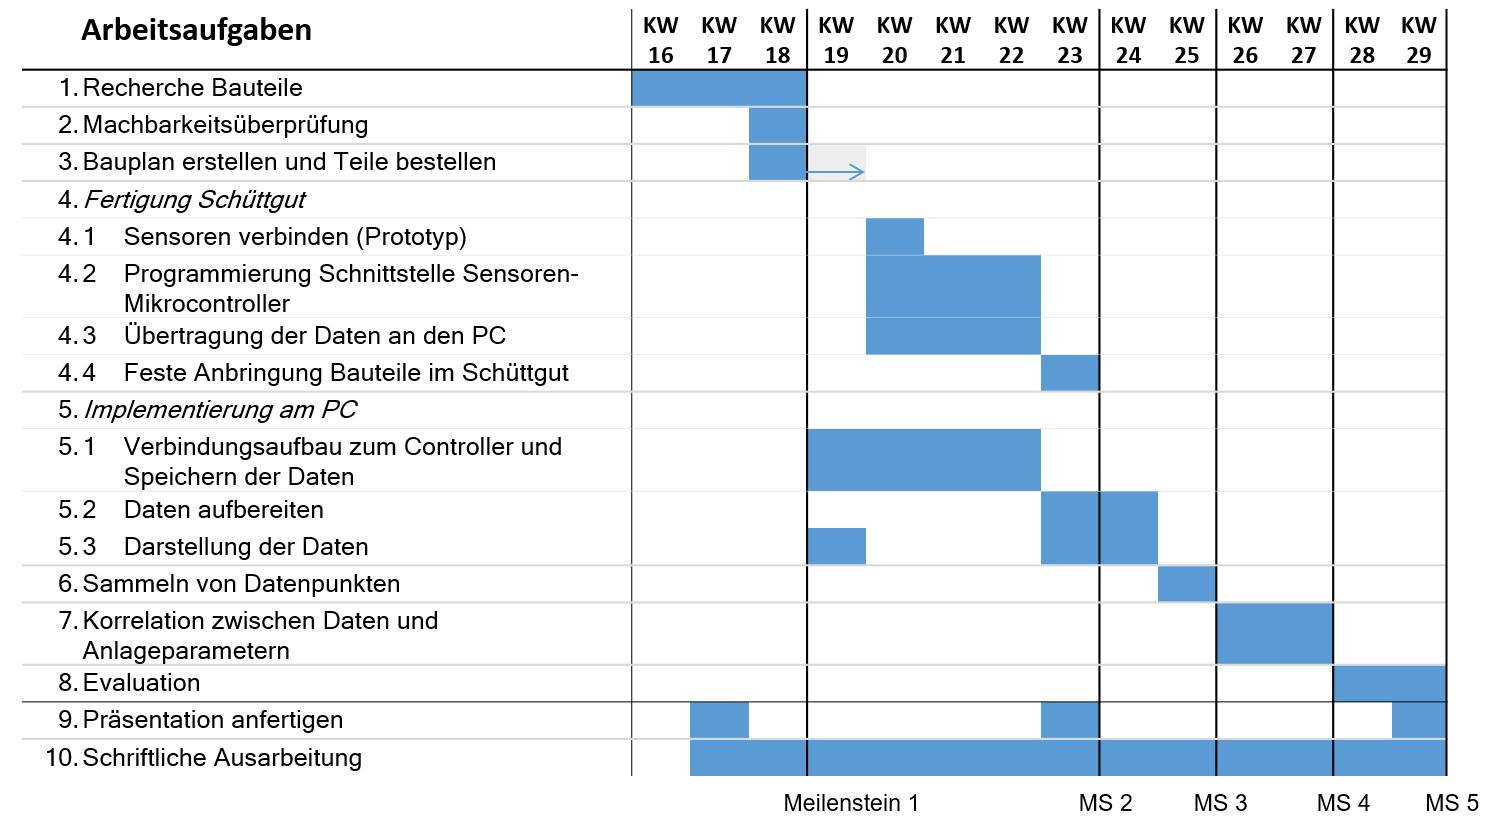
\includegraphics[width=1\textwidth]{images/k2-projektplan.JPG}
	\caption {Projektplanung runtergebrochen auf einzelne Arbeitsschritte}
	\label{fig:k2}
\end{figure}

Meilenstein 1 ist für die ersten drei Projektwochen angesetzt. Die grau markierte Kalenderwoche 19 bei Aufgabe 3 wird für die Bestelldauer der Bauteile geblockt. Solange kann nicht mit den Aufgabenteilen 4.* begonnen werden. Allerdings können einzelne Aufgaben aus Teil 5.* vorgezogen werden. Fortführend werden die Aufgaben 4 und 5 parallel bearbeitet, wobei Meilenstein 2 nach Kalenderwoche 23 ein fertiges instrumentiertes Schüttgut aufweist. Meilenstein 3 wird zwei Wochen später nach beenden von Aufgabenteil 5 und dem Sammeln von Testdaten erreicht. Ab Kalenderwoche 26 beginnt die Analyse der Daten für den Abschluss von Meilenstein 4. Die letzten beiden Wochen sind für die Evaluation des Projektes angesetzt, womit auch Meilenstein 5 erreicht wird. Zusätzlich sollte das Projekt fortlaufend dokumentiert sowie drei Präsentationen ausgearbeitet werden.